\documentclass[aps,prb,10pt,twocolumn,superscriptaddress]{revtex4-2}

\usepackage{tikz,pgf}
\usepackage{amsfonts}
\usepackage{amsmath}
\usepackage{amssymb}
\usepackage{amsthm}
\usepackage{bm}
\usepackage{mathtools}
\usepackage{braket}
\usepackage[right]{lineno}
\usepackage{algorithmicx,algpseudocode}
\usepackage[linesnumbered,ruled,vlined]{algorithm2e}
\usepackage{listings}
\usepackage{subcaption}
\usepackage{caption}
\usepackage{enumitem}
\usepackage{bbm}
\usepackage{graphicx}
\usepackage{array}
\usepackage{booktabs}
\usepackage{float}
\usepackage{hyperref}
\usepackage{xcolor}
\usepackage{todonotes}

\hypersetup{
    colorlinks=true,
    linkcolor=blue,
    citecolor=blue,
    urlcolor=blue
}

\newtheorem{theorem}{Theorem}
\newtheorem{corollary}[theorem]{Corollary}
\newtheorem{remark}[theorem]{Remark}

\newcommand{\placeholderfigure}[2]{%
\begin{figure}[t]
    \centering
    \fbox{\rule{0pt}{2.25in}\rule{0.92\linewidth}{0pt}}
    \caption{#2}
    \label{#1}
\end{figure}
}

\begin{document}

\title{Hybrid Krotov gradient descent Optimization for Quantum Machine Learning}


\author{Maximilian Fröhlich}
\affiliation{Weierstrass Institute for Applied Analysis and Stochastics, Berlin, Germany}
\email{froehlich@wias-berlin.de}
\author{Martin Eigel}
\affiliation{Weierstrass Institute for Applied Analysis and Stochastics, Berlin, Germany}
\author{Michael Hintermüller}
\affiliation{Weierstrass Institute for Applied Analysis and Stochastics, Berlin, Germany}

\date{\today}





\begin{abstract}
We introduce and study a Krotov-inspired discrete adjoint optimization scheme for quantum machine learning and focus on a hybrid online-to-batch schedule. The method transfers the forward/costate/local-update logic of continuous-time optimal control to parameterized quantum circuits by replacing time locality with gate-index locality. For a broad class of fixed-generator variational gates and terminal-state losses, we show that the batch Krotov direction coincides with the exact gradient of the empirical loss. Under standard smoothness assumptions, this yields monotonic descent and convergence of the batch method, and convergence of the tail of the hybrid method after a finite switch to the batch phase. \textcolor{red}{add numerical benchmarking here}
\end{abstract}


\maketitle
\section{Introduction}

Optimization remains one of the main bottlenecks in variational quantum algorithms and quantum machine learning \cite{CerezoEtAl2021VQA,McCleanEtAl2016Theory,MollEtAl2018QST,BiamonteEtAl2017QML,KandalaEtAl2017HEA,McCleanEtAl2018Barren,WangEtAl2021NoiseBP}. In many settings, standard first-order methods provide robust baselines but may converge slowly or require many objective and gradient evaluations, while second-order and quasi-Newton methods can yield strong late-stage refinement but may be more expensive or less naturally aligned with the structure of parameterized quantum circuits. This raises the question whether optimization rules that explicitly exploit circuit propagation structure can offer a useful alternative.

Krotov's method is a classical optimization technique from optimal control \cite{KonnovKrotov1999,WerschnikGross2007,BrifChakrabartiRabitz2010,PalaoKosloff2003,ReichNdongKoch2012,GoerzEtAl2019Krotov}. Its defining ingredients are a forward state trajectory, a backward sensitivity trajectory, and a local update rule derived from the constrained dynamical structure of the problem. In coherent quantum control, these ingredients match the physics especially naturally: the state evolves unitarily, the costate propagates backward through adjoint dynamics, and the update can be written directly in terms of inner products of propagated states and control generators. This motivates the question whether the same logic can be transferred from continuous-time control to gate-structured quantum machine learning models.

In this work we study a discrete, circuit-level adaptation of this idea \cite{SchuldEtAl2019Gradients,BanchiCrooks2021SPSR,WierichsEtAl2022ShiftRules}. The central conceptual move is to replace continuous time by gate index. Forward propagation through the circuit produces a sequence of intermediate states, backward propagation produces a sequence of costates, and local gate-wise update directions are constructed from both. We consider three variants: an online version that updates sample by sample, a batch version that averages sample-wise gate contributions over the dataset, and a hybrid method that uses online updates in an initial phase before switching to batch refinement.

The present paper has two goals. First, it formulates the method in a mathematically clean way and clarifies the extent to which the batch variant can be treated as an exact gradient method. Second, \textcolor{red}{add tested qml models and compared pennylane optimizers here}

The main contributions are as follows.
\begin{itemize}
    \item We formulate a Krotov-inspired discrete adjoint update for parameterized quantum circuits and distinguish carefully between its online, batch, and hybrid variants.
    \item We prove that for fixed-generator variational gates and terminal-state losses, the batch Krotov direction coincides with the exact gradient of the empirical loss. \textcolor{red}{which is basically a generalization of Jones and Grace gradient derivation}
    \item Under standard smoothness assumptions, we establish monotonic descent and convergence of the batch method, and convergence of the tail of the hybrid method after a finite switch to batch updates.
    \item We clarify the mechanism behind the fast initial loss decrease: the batch Krotov direction is not a hidden alternative descent direction but the exact full-batch gradient, whereas the online phase is a sequential stale-adjoint gate update that performs many local corrections within one epoch. 
    \item We perform matched hyperparameter sweeps for hybrid Krotov, \textcolor{red}{add pennylane optimizers here}. 
\end{itemize}

At the same time, we emphasize from the outset that the present method is not a literal transcription of the classical continuous-time Krotov theorem. The adaptation studied here is best understood as a structured discrete adjoint optimizer for parameterized quantum circuits. The strongest theoretical guarantees in this paper apply to the batch method and to the post-switch phase of the hybrid schedule.

\section{Related Work}

The present work sits at the intersection of quantum optimal control and variational quantum circuit optimization. Its conceptual motivation comes from Krotov-type methods, where a forward state, a backward costate, and a local structure-aware update are coupled through the underlying dynamics. In variational quantum algorithms, by contrast, optimization is usually framed in terms of generic first-order or quasi-Newton updates applied to a black-box objective over circuit parameters. Our contribution is to expose an intermediate viewpoint: the circuit is still discrete and parameterized, but the optimizer can exploit gate-local propagation structure rather than treating the loss as an opaque scalar function.

This structural viewpoint is only meaningful if it is compared against strong modern baselines. We therefore benchmark against Adam, L-BFGS-B,  quantum natural gradient (QNG) \cite{StokesEtAl2020QNG} \textcolor{red}{add ADAM, BFGS and all other pennylane optimizer references here}. The tuned comparisons below instead identify more precisely where the method helps and where it does not.

\section{From continuous-time Krotov to gate-local QML updates}

\subsection{Continuous-time Krotov in optimal control}

Krotov's method originates in constrained optimal control \cite{KonnovKrotov1999}. In the standard setting, a state variable \(\psi(t)\) evolves under a control \(\epsilon(t)\), and one seeks to minimize a cost functional of the form
\begin{equation}
J[\psi,\epsilon]
=
\Phi(\psi(T))
+
\int_0^T g_a(\epsilon(t),t)\,dt
+
\int_0^T g_b(\psi(t),t)\,dt.
\label{eq:generic_cost}
\end{equation}
In coherent quantum dynamics, \(\psi(t)\) often satisfies
\begin{equation}
i \frac{d}{dt}\psi(t)=H(\epsilon(t),t)\psi(t),
\label{eq:schrodinger}
\end{equation}
with prescribed initial condition \(\psi(0)=\psi_0\). Krotov's method constructs a new control \(\epsilon^{(i+1)}(t)\) from a current iterate \(\epsilon^{(i)}(t)\) by combining a forward propagation of the state, a backward propagation of a costate \(\chi(t)\), and a local update rule. A typical schematic form is
\begin{equation}
\epsilon^{(i+1)}(t)
=
\epsilon^{(i)}(t)
+
\frac{S(t)}{\lambda_a}
\operatorname{Im}
\left\langle
\chi^{(i)}(t)
\middle|
\frac{\partial H}{\partial \epsilon}
\middle|
\psi^{(i+1)}(t)
\right\rangle,
\label{eq:krotov_update}
\end{equation}
where \(S(t)\) is a shape function and \(\lambda_a\) is a regularization parameter. The defining conceptual feature is that the update respects the dynamical structure of the problem rather than treating the objective as a black-box function of the control \cite{SklarzTannor2002,PalaoKosloff2003,ReichNdongKoch2012,WerschnikGross2007,BrifChakrabartiRabitz2010}.

\subsection{Parameterized quantum models and terminal-state losses}

In the quantum machine learning setting considered here, the trainable model is a parameterized quantum circuit
\begin{equation}
U(\bm{\theta},x)=U_M(\theta_M,x)\cdots U_1(\theta_1,x),
\label{eq:circuit}
\end{equation}
with trainable parameters \(\bm{\theta}=(\theta_1,\dots,\theta_M)\) and input \(x\). Given a fixed initial state \(|\psi_0\rangle\), the final state for sample \(x_n\) is
\begin{equation}
|\psi_{n,M}(\bm{\theta})\rangle
=
U(\bm{\theta},x_n)|\psi_0\rangle.
\label{eq:final_state}
\end{equation}
We consider binary classification with an empirical loss
\begin{equation}
F(\bm{\theta})=\frac{1}{N}\sum_{n=1}^N L_n(\bm{\theta}),
\qquad
L_n(\bm{\theta})=\ell(p_n(\bm{\theta}),y_n),
\label{eq:empirical_loss}
\end{equation}
where \(p_n(\bm{\theta})\) is the model prediction for sample \(n\), \(y_n\in\{0,1\}\), and \(\ell\) is binary cross-entropy \cite{MitaraiEtAl2018QCL,SchuldEtAl2020CircuitCentric,PerezSalinasEtAl2020DataReupload}.

For a simple one-observable readout, we set
\begin{equation}
z_n(\bm{\theta})
=
\langle \psi_{n,M}(\bm{\theta})|O|\psi_{n,M}(\bm{\theta})\rangle,
\qquad
p_n(\bm{\theta})=\frac{z_n(\bm{\theta})+1}{2}.
\label{eq:simple_readout}
\end{equation}
More generally, if the circuit output is passed into a classical affine head,
\begin{align}
&m_{n,j}
=
\langle \psi_{n,M}(\bm{\theta})|O_j|\psi_{n,M}(\bm{\theta})\rangle,\\
&s_n=\bm{w}^{\top}\bm{m}_n+b, \\
&p_n=\sigma(s_n),
\label{eq:hybrid_head}
\end{align}
then the loss derivative propagates through the classical head before defining the terminal costate \cite{SchuldEtAl2019Gradients,BanchiCrooks2021SPSR,WierichsEtAl2022ShiftRules}.

\subsection{Gate-local forward and backward propagation}

The discrete analogue of continuous-time Krotov is obtained by replacing time locality with gate-index locality. For each sample \(n\), define forward states
\begin{equation}
|\psi_{n,0}\rangle=|\psi_0\rangle,
\qquad
|\psi_{n,k}(\bm{\theta})\rangle
=
U_k(\theta_k,x_n)\cdots U_1(\theta_1,x_n)|\psi_0\rangle,
\label{eq:forward_states}
\end{equation}
for \(k=1,\dots,M\).

Assuming the sample loss depends only on the final state, we define the terminal costate \(|\chi_{n,M}(\bm{\theta})\rangle\) by the first-variation identity
\begin{equation}
\delta L_n(\bm{\theta})
=
2\,\mathrm{Re}\,
\langle \chi_{n,M}(\bm{\theta}) \mid \delta \psi_{n,M}(\bm{\theta}) \rangle.
\label{eq:first_variation}
\end{equation}
For the simple readout \eqref{eq:simple_readout}, this yields
\begin{equation}
|\chi_{n,M}(\bm{\theta})\rangle
=
\frac{1}{2}\frac{\partial \ell}{\partial p_n}
\,O\,|\psi_{n,M}(\bm{\theta})\rangle.
\label{eq:terminal_costate_simple}
\end{equation}
For the hybrid head \eqref{eq:hybrid_head}, one obtains
\begin{equation}
|\chi_{n,M}(\bm{\theta})\rangle
=
(p_n-y_n)
\left(\sum_j w_j O_j\right)
|\psi_{n,M}(\bm{\theta})\rangle.
\label{eq:terminal_costate_hybrid}
\end{equation}

Backward-propagated costates are then defined by
\begin{equation}
|\chi_{n,k}^{\mathrm{after}}(\bm{\theta})\rangle
=
U_{k+1}(\theta_{k+1},x_n)^\dagger \cdots U_M(\theta_M,x_n)^\dagger
|\chi_{n,M}(\bm{\theta})\rangle.
\label{eq:backward_costates}
\end{equation}

\subsection{Online, batch, and hybrid Krotov}

Suppose gate \(k\) is parameterized by a scalar \(\theta_k\) and takes the form
\begin{equation}
U_k(\theta_k,x_n)=\exp\!\left(-\frac{i}{2}\alpha_k(\theta_k,x_n)G_k\right),
\label{eq:fixed_generator_gate}
\end{equation}
where \(G_k\) is a fixed Hermitian generator. The corresponding gate-local contribution for sample \(n\) is
\begin{equation}
\Delta_{n,k}(\bm{\theta})
=
\frac{\partial \alpha_k}{\partial \theta_k}(\theta_k,x_n)\,
2\,\mathrm{Re}\!\left\langle
\chi_{n,k}^{\mathrm{after}}(\bm{\theta})
\middle|
\left(-\frac{i}{2}G_k\right)
\middle|
\psi_{n,k}(\bm{\theta})
\right\rangle.
\label{eq:discrete_contribution}
\end{equation}

This can be interpreted as a generalization of the reverse-mode gradient derived in \cite{jones2020efficientcalculationgradientsclassical} and yields the same computational advantage in full quantum state simulation compared to parameter-shift rule .

For fixed \(\bm{\theta}\), the quantity \(\Delta_{n,k}(\bm{\theta})\) is exactly the sample-wise partial derivative \(\partial L_n/\partial \theta_k\). The distinction between the online and batch variants is therefore not the local formula itself, but how this formula is reused during an update sweep.

We consider three algorithmic variants.

\paragraph{Online Krotov.}
For one training sample \((x_n,y_n)\), we compute the forward states and backward costates once at a current parameter vector \(\bm{\theta}^{\mathrm{old}}\), then update parameters gate by gate. If \(|\tilde{\psi}_{n,k-1}\rangle\) denotes the forward state obtained after updating gates \(1,\dots,k-1\) within the same sample, the implemented gate-\(k\) online signal has the mixed stale/fresh form
\begin{equation}
\widehat{\Delta}_{n,k}
=
\frac{\partial \alpha_k}{\partial \theta_k}(\theta_k^{\mathrm{old}},x_n)\,
2\,\mathrm{Re}\!\left\langle
\chi_{n,k}^{\mathrm{after}}(\bm{\theta}^{\mathrm{old}})
\middle|
\left(-\frac{i}{2}G_k\right)
\middle|
U_k(\theta_k^{\mathrm{old}},x_n)\tilde{\psi}_{n,k-1}
\right\rangle,
\label{eq:online_mixed_signal}
\end{equation}
followed by \(\theta_k \leftarrow \theta_k-\eta_{\mathrm{on}}\widehat{\Delta}_{n,k}\). Thus the backward trajectory is fully stale, whereas the forward trajectory is refreshed gate by gate within the sample. This variant is aggressive and often effective in the early training regime, but it may induce substantial late-stage oscillations.

\paragraph{Batch Krotov.}
We average the sample-wise contributions over the dataset,
\begin{equation}
\bar{\Delta}_k(\bm{\theta})
=
\frac{1}{N}\sum_{n=1}^N \Delta_{n,k}(\bm{\theta}),
\label{eq:batch_direction}
\end{equation}
and perform a single parameter update
\begin{equation}
\theta_k^{(m+1)}=\theta_k^{(m)}-\eta\,\bar{\Delta}_k(\bm{\theta}^{(m)}).
\label{eq:batch_update}
\end{equation}
This is more stable than the online rule and aligns directly with the empirical loss.

\paragraph{Hybrid Krotov.}
The hybrid method uses online Krotov for an initial phase \(m<T_{\mathrm{sw}}\) and switches to batch Krotov for \(m\geq T_{\mathrm{sw}}\). The intended effect is to combine rapid basin entry with stable late-stage refinement.

\paragraph{Non-gate parameters.}
For hybrid quantum-classical models, purely classical parameters such as \(\bm{w}\) and \(b\) in \eqref{eq:hybrid_head} are not updated by the gate-local Krotov rule. In the experiments below, such parameters receive their exact loss-gradient update within the same training epoch.

\paragraph{Optional discrete scaling factors.}
The continuous-time update \eqref{eq:krotov_update} contains the multiplicative factor \(S(t)/\lambda_a\). In the discrete implementation this motivates optional per-gate factors \(S_k\) of the form
\begin{equation}
\theta_k^{+}
=
\theta_k-\eta S_k \widehat{\Delta}_{n,k}
\qquad\text{or}\qquad
\theta_k^{+}
=
\theta_k-\eta S_k \bar{\Delta}_k,
\label{eq:discrete_scaling}
\end{equation}
depending on whether the phase is online or batch. We tested both adaptive choices, where \(S_k\) depends on the current update magnitude, and metadata-based choices, where \(S_k\) depends on layer or parameter group. These factors should be interpreted as heuristic preconditioners rather than as part of the exact-gradient theory; the convergence results below apply to the unscaled batch rule.

\section{Theoretical properties}

The main theoretical message of this paper is deliberately modest. We do not claim that the present discrete QML adaptation inherits the full classical continuous-time Krotov theorem. Instead, we prove three precise statements:
\begin{enumerate}
    \item for fixed-generator gates and terminal-state losses, the batch Krotov direction is the exact gradient of the empirical loss;
    \item under standard smoothness assumptions, the batch method is a monotone gradient-descent scheme and converges to stationary points;
    \item the tail of the hybrid method converges after a finite switch to batch Krotov.
\end{enumerate}

\begin{theorem}[Exact gradient representation of the batch Krotov direction]
\label{thm:exact_gradient_krotov_main}
Let \(F(\bm{\theta})\) be defined by \eqref{eq:empirical_loss}, assume that each trainable gate has the fixed-generator form \eqref{eq:fixed_generator_gate}, and assume that each sample loss depends on the circuit only through the final state. Then the batch Krotov direction \(\bar{\Delta}(\bm{\theta})\) defined by \eqref{eq:batch_direction} coincides with the exact gradient of the empirical loss:
\[
\bar{\Delta}(\bm{\theta})=\nabla F(\bm{\theta}).
\]
\end{theorem}

\begin{theorem}[Monotonic descent and convergence of batch Krotov]
\label{thm:batch_krotov_convergence_main}
Assume that the batch Krotov direction equals \(\nabla F\), that \(F\) is bounded below, and that \(F\) is \(L\)-smooth on the relevant sublevel set. Consider the batch iteration
\[
\bm{\theta}^{(m+1)}=\bm{\theta}^{(m)}-\eta \nabla F(\bm{\theta}^{(m)})
\]
with fixed step size \(0<\eta<2/L\). Then \(F(\bm{\theta}^{(m)})\) is monotonically nonincreasing and
\[
F(\bm{\theta}^{(m+1)})
\leq
F(\bm{\theta}^{(m)})
-\eta\left(1-\frac{L\eta}{2}\right)\|\nabla F(\bm{\theta}^{(m)})\|^2.
\]
Moreover,
\[
\sum_{m=0}^{\infty}\|\nabla F(\bm{\theta}^{(m)})\|^2<\infty,
\qquad
\|\nabla F(\bm{\theta}^{(m)})\|\to 0,
\]
and every accumulation point is stationary. If, in addition, the iterates are bounded and \(F\) satisfies the Kurdyka-\L{}ojasiewicz property, then the whole sequence converges to a single stationary point.
\end{theorem}

\begin{corollary}[Convergence of the tail of hybrid Krotov]
\label{cor:hybrid_tail_main}
Assume that the iterates are generated by an arbitrary online Krotov phase for \(m<T_{\mathrm{sw}}\), and by batch Krotov for \(m\geq T_{\mathrm{sw}}\), with a finite switch time \(T_{\mathrm{sw}}<\infty\) and a step size satisfying \(0<\eta<2/L\). Under the assumptions of Theorem~\ref{thm:batch_krotov_convergence_main}, the tail sequence \((\bm{\theta}^{(m)})_{m\geq T_{\mathrm{sw}}}\) converges to a stationary point under the same boundedness and Kurdyka-\L{}ojasiewicz assumptions.
\end{corollary}

The proofs are given in Appendix~A and Appendix~B. The practical interpretation is important. The theoretical guarantees established here apply to the batch method and to the post-switch phase of the hybrid method. They do \emph{not} imply a monotonic-descent theorem for the online stale-adjoint phase, which empirically is precisely the regime where oscillations are observed.

\section{Why the online phase can decrease the loss quickly}

Theorem~\ref{thm:exact_gradient_krotov_main} has an immediate interpretive consequence. For gate-supported parameters, the batch Krotov direction is already the exact gradient of the empirical loss. Hence the fast initial improvement observed for hybrid Krotov cannot be explained by a hidden superior batch descent direction. The mechanism must lie in the online phase and in the way that phase reuses forward and backward information.

Equation~\eqref{eq:online_mixed_signal} shows that the implemented online rule is a mixed stale/fresh update. For the first gate of a given sample, the signal coincides with the exact sample gradient at the current parameter vector. After that first gate update, however, the forward state has already been modified while the backward costates are still those of the old parameters. The online phase is therefore best understood as a sequential Gauss-Seidel-like discrete adjoint sweep rather than as simultaneous gradient descent.

This has a simple but important algorithmic consequence. With \(N\) training samples and \(K\) gate-supported parameters, one online epoch performs \(N\times K\) local parameter modifications, because each sample triggers a full gate sweep. By contrast, the batch rule aggregates all samples before a single outer update. The online phase therefore has much finer within-epoch resolution: corrections made at early gates immediately affect the forward states seen by later gates in the same sample, and the next sample starts from the already-updated parameter vector.

This finer resolution does not require \(N\times K\) fresh adjoint recomputations. For a fixed sample, the online rule forms one forward trajectory and one backward costate trajectory and then reuses them across the whole gate sweep, so the additional gate-local corrections are mostly cheap local linear-algebra operations rather than new propagation passes. In the cost accounting used in this paper, online Krotov therefore spends roughly one sample forward pass plus one sample backward pass per training sample and amortizes that information over many sequential local updates. Adam and full-batch Krotov, by contrast, spend a full-batch forward/backward evaluation to construct one averaged update direction at the current parameter vector, while L-BFGS-B may require several such full-batch evaluations because of its line-search and quasi-Newton bookkeeping.

The price of this granularity is that the online signal is no longer the exact coordinate gradient of the current partially updated parameter vector. Under local smoothness, the mismatch between \(\widehat{\Delta}_{n,k}\) and the exact coordinate gradient after the previous intra-sample updates is controlled by the accumulated earlier gate changes, so the discrepancy is largest when the online updates are large and shrinks as the trajectory settles. We interpret this as an implicit gradient perturbation of the sequential rule, not as a proved monotonicity mechanism. In particular, the classical continuous-time Krotov theorem does not transfer to this stale-adjoint online phase.

At the sample level, the method also behaves like a structured stochastic optimizer: training samples are processed in random order, and each sample sees parameters left behind by the previous one. The online phase thus combines sample-wise stochasticity with gate-wise sequentiality. This is exactly the behavior that the switch and hyperparameter sweeps below probe. Our expectation, confirmed empirically, is that the decisive knobs are the duration of the online phase and the relative scales of the online and batch step sizes, whereas additional discrete scaling factors \(S_k\) can only provide secondary refinements.

\section{Numerical experiments}

We now examine whether the hybrid Krotov schedule remains competitive once its hyperparameters are tuned against strong optimizer baselines on fixed circuit architectures. The numerical study is deliberately organized around \emph{matched model comparisons}: for each benchmark we first fix one concrete quantum model and one concrete loss, then run independent hyperparameter sweeps for each optimizer family on exactly that same task. The figures below report, for each optimizer family, the \emph{best tested hyperparameter configuration} and show the mean training loss over the available random seeds together with one-standard-deviation bands. The horizontal axis is the accepted outer iteration count of the optimizer; for native L-BFGS-B this count refers to accepted SciPy iterations rather than internal line-search probes.

All parity and Perez--Salinas figures included in this paper were generated directly from the experiment outputs in the repository and copied into the paper folder so that the \LaTeX{} source is self-contained. Throughout, we took care to avoid the data-leakage issue encountered in an early parity prototype: training and test sets are now disjoint at the level of unique samples.

\subsection{Leakage-safe parity benchmark}

Our first benchmark is the four-bit parity classifier from the PennyLane variational-classifier demo, but implemented in both the native optimizer pipeline and a matched PennyLane reference implementation. The quantum model uses four qubits, basis-state encoding of the four-bit input, two repeated variational layers, and measurement of \(\langle Z_0\rangle\) followed by a trainable scalar bias. Each layer applies a three-parameter single-qubit Euler rotation on every qubit and then the CNOT ring
\[
0\rightarrow1,\qquad
1\rightarrow2,\qquad
2\rightarrow3,\qquad
3\rightarrow0.
\]
The labels are \(y\in\{-1,+1\}\) with odd parity mapped to \(+1\), and the objective is the mean squared error used in the original demo. To prevent trivial leakage through duplicated truth-table entries, we use a split of \(10\) unique training bit strings and \(6\) unique test bit strings from the \(16\) possible inputs.

For this model we tuned hybrid Krotov, native L-BFGS-B, and the PennyLane optimizers Adam, Adagrad, gradient descent, momentum, Nesterov momentum, RMSProp, SPSA, QNG, and Rotosolve. Every hyperparameter configuration was run with three seeds. The plotted parity curves therefore compare the best configuration \emph{within each optimizer family} rather than default settings.

\begin{figure*}[t]
    \centering
    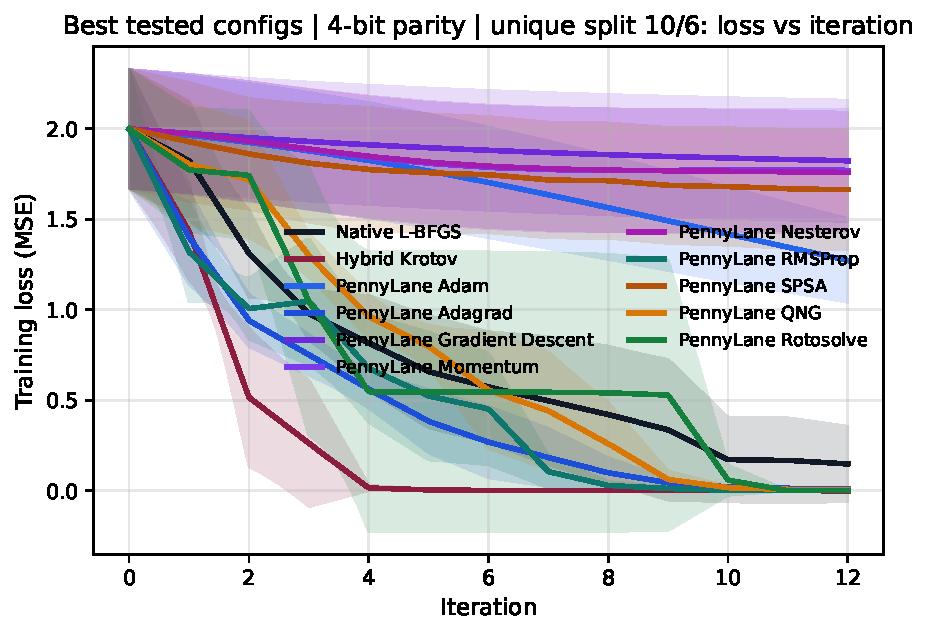
\includegraphics[width=\textwidth]{figures/parity_loss_vs_iteration.pdf}
    \caption{Leakage-safe four-bit parity benchmark. Shown are the best tested hyperparameter settings of each optimizer family. Curves denote the mean training loss over three seeds; shaded bands indicate one standard deviation. The native L-BFGS-B curve is recorded in accepted outer iterations, so it is directly comparable to the first-order and Krotov schedules.}
    \label{fig:parity-loss-iteration}
\end{figure*}

Figure~\ref{fig:parity-loss-iteration} shows three distinct regimes. First, hybrid Krotov, PennyLane RMSProp, PennyLane QNG, and PennyLane Rotosolve all solve the leakage-safe task at their best settings, with hybrid Krotov and Rotosolve reaching the smallest final losses in the tested budget. Second, the tuned first-order baselines separate sharply: RMSProp and Adagrad are clearly the strongest practical PennyLane baselines, whereas Adam, plain gradient descent, momentum, Nesterov, and SPSA remain substantially weaker on this benchmark. Third, native L-BFGS-B is \emph{not} a dominant method on this discrete parity task; after correcting the trace accounting to compare only accepted optimizer iterations, its best tested configuration remains below the best Krotov and PennyLane contenders in both final loss and test accuracy.

The parity experiment is important mainly as a controlled calibration problem. Because the model is small and the loss is exactly matched between the native and PennyLane implementations, it isolates optimizer behavior from architecture confounders. In this setting the hybrid Krotov schedule is highly competitive already after a modest number of iterations, while the strongest PennyLane baselines remain RMSProp, QNG, and Rotosolve rather than Adam.

\subsection{Perez--Salinas data re-uploading benchmark}

Our second benchmark is substantially less toy-like and uses the data re-uploading classifier of Perez-Salinas \emph{et al.} on the two-dimensional \texttt{crown} classification problem. The circuit is the entangling four-qubit, eight-layer re-uploading model with the affine classical readout head enabled. Inputs are continuous points in \([-1,1]^2\), embedded repeatedly across the circuit, and the loss is the weighted-fidelity objective used in our native implementation and mirrored exactly in the PennyLane reference model. For this experiment we generated \(600\) samples per split, yielding \(420\) training and \(180\) test points under a \(70/30\) split. Since the data are sampled continuously, train/test duplication is not structurally expected; we nevertheless enforced a disjoint split in the benchmark scripts.

The optimizer comparison was again based on tuned families rather than defaults. We swept hybrid Krotov and the PennyLane optimizers Adam, Adagrad, gradient descent, momentum, Nesterov momentum, RMSProp, and SPSA with three seeds per hyperparameter combination. We also include native L-BFGS-B, truncated to the same \(20\)-iteration budget in the merged report and figure. A preliminary QNG study was performed separately, but full-metric QNG requires an auxiliary wire on this model and the block-diagonal variant was already much more expensive and not competitive enough to justify inclusion in the final large sweep.

\begin{figure*}[t]
    \centering
    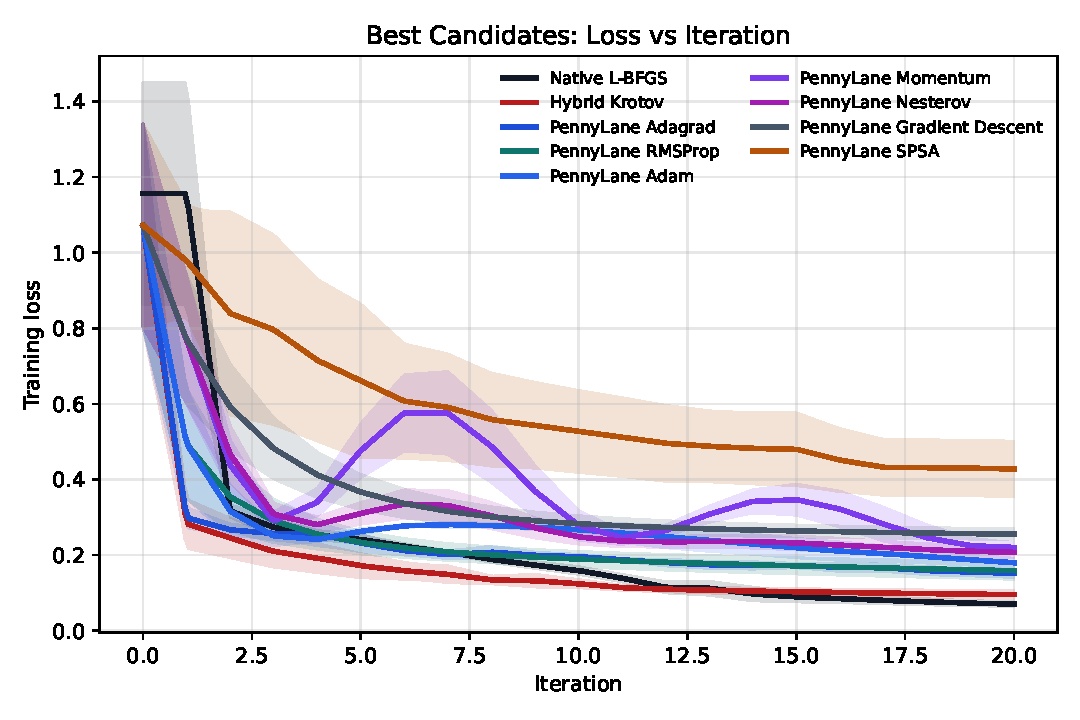
\includegraphics[width=\textwidth]{figures/perez_salinas_loss_vs_iteration.pdf}
    \caption{Perez--Salinas data re-uploading benchmark on the \texttt{crown} problem. Each curve shows the best tested hyperparameter configuration of one optimizer family. Means and standard deviations are computed over the available seeds for that configuration; native L-BFGS-B is shown at the same \(20\)-iteration budget used in the sweep comparison.}
    \label{fig:perez-loss-iteration}
\end{figure*}

The behavior in Fig.~\ref{fig:perez-loss-iteration} is qualitatively different from the parity task and more informative for the intended QML application regime. Native L-BFGS-B is the strongest method at the common \(20\)-step budget, reaching the lowest loss and the highest test accuracy in the merged comparison. Hybrid Krotov is nevertheless the best-performing method among the newly tuned three-seed sweep results and remains markedly stronger than the tuned PennyLane first-order baselines. Among those baselines, Adagrad and RMSProp emerge as the best choices, with Adam close behind but consistently weaker at its best tested setting. Momentum, Nesterov, plain gradient descent, and SPSA are clearly dominated.

Quantitatively, the best merged Perez--Salinas configurations are as follows. Native L-BFGS-B reaches mean test accuracy \(0.95\) and mean final loss \(0.0706\) at the \(20\)-iteration cutoff. The best hybrid Krotov setting reaches mean test accuracy \(0.9352\) and mean final loss \(0.0954\). The best PennyLane baselines remain well below this level: Adagrad attains mean test accuracy \(0.8315\) with mean final loss \(0.1517\), RMSProp attains \(0.8204\) and \(0.1587\), and Adam attains \(0.8185\) and \(0.1797\). Thus the tuned hybrid Krotov schedule does not beat the strongest quasi-Newton baseline on this model, but it does substantially outperform the tuned PennyLane first-order methods in the same experiment design.

\subsection{Interpretation}

Taken together, the two benchmarks support a consistent interpretation of the method. On the small parity task, several optimizers can solve the problem when sufficiently tuned, and the main value of the comparison is to confirm that hybrid Krotov remains competitive under a leakage-safe protocol and against matched PennyLane implementations. On the more structured Perez--Salinas re-uploading task, the separation between optimizers becomes clearer: native L-BFGS-B is the strongest method at fixed iteration budget, hybrid Krotov is the strongest method among the newly tuned sweep families, and the best PennyLane baselines are Adagrad and RMSProp rather than Adam.

These findings are consistent with the theoretical picture developed above. The late-stage batch phase of hybrid Krotov is an exact full-batch gradient method on the gate-supported parameters, while the online phase provides an aggressive structured preconditioning effect during the early iterations. Empirically this combination is sufficient to close much of the gap to L-BFGS-B and to outperform a wide range of tuned first-order baselines, but it does not universally dominate a strong quasi-Newton method on every architecture. This is precisely the kind of outcome one would expect from a practically useful structured optimizer rather than a universal winner.

\section{Discussion}


\section{Conclusion}



\section*{Acknowledgments}
% TODO: Add acknowledgments.

\bibliography{bib.bib}

\appendix

\section{Proof of the exact-gradient representation theorem}

\begin{theorem}[Exact gradient representation of the batch Krotov direction]
\label{thm:exact_gradient_krotov_appendix}
Let
\[
F(\bm{\theta})=\frac{1}{N}\sum_{n=1}^N L_n(\bm{\theta})
\]
be the empirical loss of a parametrized quantum model, where for each sample \(n\),
\[
L_n(\bm{\theta})=\ell\bigl(p_n(\bm{\theta}),y_n\bigr)
\]
and the final quantum state is
\[
|\psi_{n,M}(\bm{\theta})\rangle
=
U_M(\theta_M)\cdots U_1(\theta_1)|\psi_{n,0}\rangle.
\]
For \(k=1,\dots,M\), define the forward states
\[
|\psi_{n,k}(\bm{\theta})\rangle
=
U_k(\theta_k)\cdots U_1(\theta_1)|\psi_{n,0}\rangle,
\qquad
|\psi_{n,0}(\bm{\theta})\rangle:=|\psi_{n,0}\rangle.
\]

Assume that each trainable gate is of the form
\[
U_k(\theta_k)=\exp\!\left(-\frac{i}{2}\alpha_k(\theta_k,x_n)\,G_k\right),
\]
where \(G_k\) is a fixed Hermitian operator, independent of \(\theta_k\), and
\(\alpha_k(\theta_k,x_n)\) is continuously differentiable in \(\theta_k\).

Assume furthermore that, for each sample \(n\), the loss \(L_n(\bm{\theta})\) depends on the
circuit only through the final state \( |\psi_{n,M}(\bm{\theta})\rangle \), and that the terminal costate
\[
|\chi_{n,M}(\bm{\theta})\rangle
\]
is defined by the first-variation identity
\[
\delta L_n(\bm{\theta})
=
2\,\mathrm{Re}\,\langle \chi_{n,M}(\bm{\theta})\mid \delta\psi_{n,M}(\bm{\theta})\rangle
\]
for every variation \(|\delta\psi_{n,M}(\bm{\theta})\rangle\) of the final state.

Finally, define the backward-propagated costates
\[
|\chi_{n,k}^{\mathrm{after}}(\bm{\theta})\rangle
=
U_{k+1}(\theta_{k+1})^\dagger\cdots U_M(\theta_M)^\dagger
|\chi_{n,M}(\bm{\theta})\rangle,
\qquad k=1,\dots,M.
\]

Then, for every sample \(n\) and every gate parameter \(\theta_k\),
\[
\frac{\partial L_n}{\partial \theta_k}(\bm{\theta})
=
2\,\mathrm{Re}\!\left\langle
\chi_{n,k}^{\mathrm{after}}(\bm{\theta})
\middle|
\frac{\partial U_k}{\partial \theta_k}(\theta_k)
\middle|
\psi_{n,k-1}(\bm{\theta})
\right\rangle.
\]
Equivalently,
\[
\frac{\partial L_n}{\partial \theta_k}(\bm{\theta})
=
\frac{\partial \alpha_k}{\partial \theta_k}(\theta_k,x_n)\,
2\,\mathrm{Re}\!\left\langle
\chi_{n,k}^{\mathrm{after}}(\bm{\theta})
\middle|
\left(-\frac{i}{2}G_k\right)
\middle|
\psi_{n,k}(\bm{\theta})
\right\rangle.
\]
Consequently, the batch Krotov direction
\[
d_k(\bm{\theta})
:=
\frac{1}{N}\sum_{n=1}^N
\frac{\partial \alpha_k}{\partial \theta_k}(\theta_k,x_n)\,
2\,\mathrm{Re}\!\left\langle
\chi_{n,k}^{\mathrm{after}}(\bm{\theta})
\middle|
\left(-\frac{i}{2}G_k\right)
\middle|
\psi_{n,k}(\bm{\theta})
\right\rangle
\]
coincides with the exact partial derivative of the empirical loss:
\[
d_k(\bm{\theta})=\frac{\partial F}{\partial \theta_k}(\bm{\theta}).
\]
Hence
\[
d(\bm{\theta})=\nabla F(\bm{\theta}).
\]
\end{theorem}

\begin{proof}
The proof adapts the reverse-mode gradient derivation of \cite{jones2020efficientcalculationgradientsclassical} from expectation-value objectives to sample-wise terminal-state losses and their empirical average
Fix a sample $n$ and a parameter index $k$.
By definition of the forward states,
\[
|\psi_{n,M}(\bm{\theta})\rangle
=
U_M(\theta_M)\cdots U_{k+1}(\theta_{k+1})
U_k(\theta_k)
|\psi_{n,k-1}(\bm{\theta})\rangle.
\]
Differentiating with respect to \(\theta_k\) yields
\[
\frac{\partial}{\partial \theta_k}|\psi_{n,M}(\bm{\theta})\rangle
=
U_M(\theta_M)\cdots U_{k+1}(\theta_{k+1})
\frac{\partial U_k}{\partial \theta_k}(\theta_k)
|\psi_{n,k-1}(\bm{\theta})\rangle.
\]

Since \(L_n(\bm{\theta})\) depends on the circuit only through the final state and the terminal
costate is defined by
\[
\delta L_n(\bm{\theta})
=
2\,\mathrm{Re}\,\langle \chi_{n,M}(\bm{\theta})\mid \delta\psi_{n,M}(\bm{\theta})\rangle,
\]
we may apply this identity to the variation induced by changing \(\theta_k\). Thus
\[
\frac{\partial L_n}{\partial \theta_k}(\bm{\theta})
=
2\,\mathrm{Re}\!\left\langle
\chi_{n,M}(\bm{\theta})
\middle|
\frac{\partial \psi_{n,M}}{\partial \theta_k}(\bm{\theta})
\right\rangle.
\]
Substituting the previous expression gives
\[
\frac{\partial L_n}{\partial \theta_k}(\bm{\theta})
=
2\,\mathrm{Re}\!\left\langle
\chi_{n,M}(\bm{\theta})
\middle|
U_M(\theta_M)\cdots U_{k+1}(\theta_{k+1})
\frac{\partial U_k}{\partial \theta_k}(\theta_k)
\middle|
\psi_{n,k-1}(\bm{\theta})
\right\rangle.
\]

Now use the definition of the backward-propagated costate:
\[
|\chi_{n,k}^{\mathrm{after}}(\bm{\theta})\rangle
=
U_{k+1}(\theta_{k+1})^\dagger\cdots U_M(\theta_M)^\dagger
|\chi_{n,M}(\bm{\theta})\rangle.
\]
Taking adjoints yields
\[
\langle \chi_{n,M}(\bm{\theta})|
\,U_M(\theta_M)\cdots U_{k+1}(\theta_{k+1})
=
\langle \chi_{n,k}^{\mathrm{after}}(\bm{\theta})|,
\]
hence
\[
\frac{\partial L_n}{\partial \theta_k}(\bm{\theta})
=
2\,\mathrm{Re}\!\left\langle
\chi_{n,k}^{\mathrm{after}}(\bm{\theta})
\middle|
\frac{\partial U_k}{\partial \theta_k}(\theta_k)
\middle|
\psi_{n,k-1}(\bm{\theta})
\right\rangle.
\]

Now use the gate parametrization
\[
U_k(\theta_k)=\exp\!\left(-\frac{i}{2}\alpha_k(\theta_k,x_n)\,G_k\right).
\]
Because \(G_k\) is independent of \(\theta_k\), the \(\theta_k\)-dependence enters only through
the scalar function \(\alpha_k(\theta_k,x_n)\). Hence the exponent is of the form
\(f(\theta_k)G_k\) with fixed operator \(G_k\), so \(G_k\) commutes with the exponent.
Therefore
\[
\frac{\partial U_k}{\partial \theta_k}(\theta_k)
=
\frac{\partial \alpha_k}{\partial \theta_k}(\theta_k,x_n)
\left(-\frac{i}{2}G_k\right)
U_k(\theta_k).
\]
Substituting this identity yields
\begin{align*}
\frac{\partial L_n}{\partial \theta_k}(\bm{\theta})
&=
\frac{\partial \alpha_k}{\partial \theta_k}(\theta_k,x_n)\,
2\,\mathrm{Re}\!\left\langle
\chi_{n,k}^{\mathrm{after}}(\bm{\theta})
\middle|
\left(-\frac{i}{2}G_k\right)U_k(\theta_k)
\middle|
\psi_{n,k-1}(\bm{\theta})
\right\rangle \\
&=
\frac{\partial \alpha_k}{\partial \theta_k}(\theta_k,x_n)\,
2\,\mathrm{Re}\!\left\langle
\chi_{n,k}^{\mathrm{after}}(\bm{\theta})
\middle|
\left(-\frac{i}{2}G_k\right)
\middle|
\psi_{n,k}(\bm{\theta})
\right\rangle,
\end{align*}
because
\[
|\psi_{n,k}(\bm{\theta})\rangle
=
U_k(\theta_k)|\psi_{n,k-1}(\bm{\theta})\rangle.
\]
This proves the sample-wise identity.

Finally, average over \(n=1,\dots,N\). Since
\[
F(\bm{\theta})=\frac{1}{N}\sum_{n=1}^N L_n(\bm{\theta}),
\]
linearity of differentiation gives
\[
\frac{\partial F}{\partial \theta_k}(\bm{\theta})
=
\frac{1}{N}\sum_{n=1}^N \frac{\partial L_n}{\partial \theta_k}(\bm{\theta}).
\]
Substituting the established formula for each \(\partial L_n/\partial \theta_k\) yields
\[
\frac{\partial F}{\partial \theta_k}(\bm{\theta})=d_k(\bm{\theta}).
\]
Since this holds for every \(k=1,\dots,M\), it follows that
\[
d(\bm{\theta})=\nabla F(\bm{\theta}).
\]
\end{proof}

\begin{remark}
The derivative formula
\[
\frac{\partial U_k}{\partial \theta_k}
=
\frac{\partial \alpha_k}{\partial \theta_k}
\left(-\frac{i}{2}G_k\right)U_k
\]
relies on the fact that \(G_k\) is fixed and independent of \(\theta_k\). If the generator itself
depends on \(\theta_k\), then one must use the general derivative formula for operator exponentials,
and the present proof no longer applies in this form.

Likewise, the first-variation identity
\[
\delta L_n(\bm{\theta})
=
2\,\mathrm{Re}\,\langle \chi_{n,M}(\bm{\theta})\mid \delta\psi_{n,M}(\bm{\theta})\rangle
\]
is valid in the present form because the loss depends only on the final state. If the objective
contains explicit dependence on intermediate states, mid-circuit measurements, or trajectory-level
regularization terms, then the corresponding adjoint construction must be modified.
\end{remark}

\section{Proof of the convergence theorem and hybrid corollary}

\begin{theorem}[Monotonic descent and convergence of batch Krotov]
\label{thm:batch_krotov_convergence_appendix}
Let
\[
F(\bm{\theta})=\frac{1}{N}\sum_{n=1}^N \ell_n(\bm{\theta}), \qquad \bm{\theta}\in\mathbb{R}^p,
\]
be the empirical loss of a parametrized quantum model. Assume that:
\begin{enumerate}
    \item \(F\) is bounded from below;
    \item \(F\) is \(L\)-smooth on the sublevel set
    \[
    \mathcal{L}_0:=\{\bm{\theta}\in\mathbb{R}^p : F(\bm{\theta})\leq F(\bm{\theta}^{(0)})\},
    \]
    i.e.
    \[
    \|\nabla F(\bm{\theta})-\nabla F(\bm{\vartheta})\|
    \leq
    L\|\bm{\theta}-\bm{\vartheta}\|
    \qquad
    \forall \bm{\theta},\bm{\vartheta}\in\mathcal{L}_0;
    \]
    \item the batch Krotov direction coincides with the exact gradient of \(F\).
\end{enumerate}

Consider the batch Krotov iteration
\[
\bm{\theta}^{(m+1)}
=
\bm{\theta}^{(m)}-\eta \nabla F(\bm{\theta}^{(m)}),
\]
with fixed step size \(0<\eta<2/L\).

Then
\begin{enumerate}
    \item[\rm(i)] \(F(\bm{\theta}^{(m)})\) is monotonically nonincreasing and
    \[
    F(\bm{\theta}^{(m+1)})
    \leq
    F(\bm{\theta}^{(m)})
    -
    \eta\left(1-\frac{L\eta}{2}\right)\|\nabla F(\bm{\theta}^{(m)})\|^2;
    \]
    \item[\rm(ii)]
    \[
    \sum_{m=0}^{\infty}\|\nabla F(\bm{\theta}^{(m)})\|^2<\infty;
    \]
    \item[\rm(iii)]
    \[
    \|\nabla F(\bm{\theta}^{(m)})\|\to 0
    \qquad \text{as } m\to\infty;
    \]
    \item[\rm(iv)] every accumulation point of \((\bm{\theta}^{(m)})_{m\geq 0}\) is stationary.
\end{enumerate}
If, in addition, the sequence \((\bm{\theta}^{(m)})_{m\geq 0}\) is bounded and \(F\) satisfies the Kurdyka-\L{}ojasiewicz property on \(\mathcal{L}_0\), then the whole sequence converges to a single stationary point.
\end{theorem}

\begin{proof}
By Assumption (iii), the batch Krotov iteration is exactly gradient descent:
\[
\bm{\theta}^{(m+1)}=\bm{\theta}^{(m)}-\eta \nabla F(\bm{\theta}^{(m)}).
\]
Since \(F\) is \(L\)-smooth on \(\mathcal{L}_0\), the descent lemma gives
\[
F(\bm{\theta}^{(m+1)})
\leq
F(\bm{\theta}^{(m)})
+
\langle \nabla F(\bm{\theta}^{(m)}),\bm{\theta}^{(m+1)}-\bm{\theta}^{(m)}\rangle
+
\frac{L}{2}\|\bm{\theta}^{(m+1)}-\bm{\theta}^{(m)}\|^2.
\]
Substituting
\[
\bm{\theta}^{(m+1)}-\bm{\theta}^{(m)}=-\eta \nabla F(\bm{\theta}^{(m)}),
\]
we obtain
\begin{align*}
F(\bm{\theta}^{(m+1)})
&\leq
F(\bm{\theta}^{(m)})
-
\eta\|\nabla F(\bm{\theta}^{(m)})\|^2
+
\frac{L\eta^2}{2}\|\nabla F(\bm{\theta}^{(m)})\|^2 \\
&=
F(\bm{\theta}^{(m)})
-
\eta\left(1-\frac{L\eta}{2}\right)\|\nabla F(\bm{\theta}^{(m)})\|^2.
\end{align*}
Because \(0<\eta<2/L\), the coefficient
\[
c:=\eta\left(1-\frac{L\eta}{2}\right)
\]
is strictly positive. This proves (i).

Summing from \(m=0\) to \(M\) yields
\[
F(\bm{\theta}^{(M+1)})
\leq
F(\bm{\theta}^{(0)})-c\sum_{m=0}^M \|\nabla F(\bm{\theta}^{(m)})\|^2.
\]
Since \(F\) is bounded below, say by \(F_{\inf}\), we obtain
\[
c\sum_{m=0}^M \|\nabla F(\bm{\theta}^{(m)})\|^2
\leq
F(\bm{\theta}^{(0)})-F_{\inf}.
\]
Letting \(M\to\infty\) gives
\[
\sum_{m=0}^{\infty}\|\nabla F(\bm{\theta}^{(m)})\|^2<\infty,
\]
which proves (ii). In particular,
\[
\|\nabla F(\bm{\theta}^{(m)})\|\to 0,
\]
which proves (iii).

Now let \(\bm{\theta}^{\star}\) be an accumulation point. Then there exists a subsequence
\[
\bm{\theta}^{(m_j)}\to \bm{\theta}^{\star}.
\]
Since \(\nabla F\) is continuous,
\[
\nabla F(\bm{\theta}^{\star})
=
\lim_{j\to\infty}\nabla F(\bm{\theta}^{(m_j)})
=
0,
\]
using (iii). Hence \(\bm{\theta}^{\star}\) is stationary, proving (iv).

If the iterates are bounded and \(F\) satisfies the Kurdyka-\L{}ojasiewicz property, the standard KL convergence theorem for descent methods applies, yielding convergence of the entire sequence to a single stationary point.
\end{proof}

\begin{corollary}[Convergence of hybrid Krotov after a finite switch]
\label{cor:hybrid_krotov_convergence_appendix}
Let \((\bm{\theta}^{(m)})_{m\geq 0}\) be generated by a hybrid Krotov method such that there exists a finite switching time \(T<\infty\) with the following property:
\begin{itemize}
    \item for \(m<T\), the iterates are generated by an arbitrary online Krotov phase;
    \item for \(m\geq T\), the iterates are generated by the batch Krotov update
    \[
    \bm{\theta}^{(m+1)}
    =
    \bm{\theta}^{(m)}-\eta \nabla F(\bm{\theta}^{(m)}),
    \]
    with a step size \(0<\eta<2/L\).
\end{itemize}
Assume that the assumptions of Theorem~\ref{thm:batch_krotov_convergence_appendix} hold on the sublevel set
\[
\mathcal{L}_T:=\{\bm{\theta}\in\mathbb{R}^p : F(\bm{\theta})\leq F(\bm{\theta}^{(T)})\}.
\]
Then the tail sequence \((\bm{\theta}^{(m)})_{m\geq T}\) converges to a stationary point under the same boundedness and Kurdyka-\L{}ojasiewicz assumptions.
\end{corollary}

\begin{proof}
Define the shifted sequence
\[
\widetilde{\bm{\theta}}^{(j)}:=\bm{\theta}^{(T+j)}, \qquad j\geq 0.
\]
By construction,
\[
\widetilde{\bm{\theta}}^{(j+1)}
=
\widetilde{\bm{\theta}}^{(j)}-\eta \nabla F(\widetilde{\bm{\theta}}^{(j)}),
\]
with \(0<\eta<2/L\). Thus \((\widetilde{\bm{\theta}}^{(j)})_{j\geq 0}\) is exactly a batch Krotov sequence started from \(\widetilde{\bm{\theta}}^{(0)}=\bm{\theta}^{(T)}\). Applying Theorem~\ref{thm:batch_krotov_convergence_appendix} to the shifted sequence proves the claim.
\end{proof}

\end{document}
